% Préambule APMEP - Annales
% Auteurs
% tapuscrit : 			Mathieu Drillet
% relecture : Hubert proton
% figures TikZ :
% figures pstricks :
% modifications :
% Remerciements :
% version 0 : 2026-06-30
%
\documentclass[12pt,a4paper,french]{article}

% Packages
%%% codage et police utilisée
\usepackage[T1]{fontenc}
\RequirePackage{iftex}
\iftutex % moteur utf-8 lualatex, xelatex
	\usepackage{fourier-otf} % remplace fourier pour moteur utf8 (LuaLaTeX, XeLaTeX)
	% Alternatives nécéssite (LuaLaTeX, XeLaTeX)
    \usepackage{hyperref}
	%\usepackage{fontspec}% pour utiliser des fontes système
\else % pour les autres moteurs latex, pdflatex
	\usepackage[utf8]{inputenc}
	\usepackage{fourier}
	\usepackage{amsmath,amssymb}
    \usepackage[dvips]{hyperref}
    \renewcommand{\ttdefault}{lmtt}
\fi
\usepackage[normalem]{ulem}
\usepackage{pifont}
\usepackage{lscape}
% tableaux
\usepackage{multicol}
\usepackage{multirow}
\usepackage{tabularx}
\usepackage{tabularray}
% texte et composition
\usepackage{textcomp}
\usepackage{babel}
\DecimalMathComma
\usepackage[np]{numprint}
%
\usepackage{fancyhdr}
\usepackage{makeidx}
\makeindex
% pour le symbole €
\usepackage{eurosym}
\DeclareRobustCommand{\officialeuro}{%
  \ifmmode\expandafter\text\fi
  {\fontencoding{U}\fontfamily{eurosym}\selectfont e}}
\AtBeginDocument{\renewcommand{\euro}{\officialeuro}}
% couleurs étendues
\usepackage{xcolor}
% pour les listes
\usepackage{enumitem}
% Enumérations réglage par défaut
\setlist[itemize]{label=\textbullet,leftmargin=5mm,labelwidth=3mm,labelsep=2mm,align=left}
\setlist[enumerate]{labelindent=0pt, leftmargin=5mm, labelsep=2mm, labelwidth=3mm,labelsep=2mm, align= left}
\setlist[enumerate,1]{label = \textbf{\arabic*.}}
\setlist[enumerate,2]{label = \textbf{\alph*.}}
\setlist[enumerate,3]{label = \textbf{\roman*.}}
% pour l'ajustement des boites (figures…)
\usepackage{adjustbox}
% pour ne pas commencer un exercice en fin de page
\usepackage{needspace}
%
% Taille de la zone d'écriture
\usepackage[left=1.5cm,right=1.5cm,top=3cm,bottom=3cm]{geometry}
\setlength{\headheight}{15pt}
%
% Formatage du pdf
\hypersetup{%
    pdfauthor = {APMEP},
    pdfsubject = {Troisième, générale},
    pdftitle = {Brevet des collèges -- Session 2026 -- },
    allbordercolors = white,
    pdfstartview=FitH
}
% Pour scratch (code)
\usepackage{scratch3}
% Pour le code Python
\usepackage{listings}
\lstdefinestyle{python}{
  language=Python,
  basicstyle=\ttfamily\small,
  keywordstyle=\color{blue}\bfseries,
  commentstyle=\color{gray}\itshape,
  stringstyle=\color{orange},
  numbers=left,
  numberstyle=\tiny\color{gray},
  breaklines=true,
  frame=single,
  backgroundcolor=\color{gray!5},
  tabsize=4
}
  % usage (exemple)
  %\begin{lstlisting}[style=python]
%def seuil():
%    n = 1
%    p = 0.5
%    while p < 0.6 :
%       n = n + 1
%       p = p*7/15 + 1/3
%    return n
%\end{lstlisting}


% Pour une visualisation de type tableur
\usepackage{pas-tableur}
%
%% pour PsTricks
\usepackage{pst-bezier}%% AVANT les autres PST
\usepackage{pstricks-add}
%\usepackage{pst-func,pst-tree,pst-circ}
\usepackage{pst-eucl}
%% pour TikZ
\usepackage{tikz,pgfplots,pgf,tkz-tab,tikzpagenodes}
\usetikzlibrary{calc,patterns,decorations,arrows.meta,patterns.meta,arrows}
\pgfplotsset{compat=1.18,/pgf/number format/.cd,use comma}
\usepackage{icomma} % gestion des espaces autour des virgules
\DeclareMathSymbol{;}{\mathbin}{operators}{"3B}% pour un espacement correct du ; en mode maths
%%%%%%%%%%%%%%%%%%%%%%%%%%%%%%%%%%%%%%%%%%
% Définitions
%
% notation en mode mathématique et hors mode mathématique
\newcommand{\R}{\ensuremath{\mathbb{R}}} 
\newcommand{\N}{\ensuremath{\mathbb{N}}}
\newcommand{\D}{\ensuremath{\mathbb{D}}}
\newcommand{\Z}{\ensuremath{\mathbb{Z}}}
\newcommand{\Q}{\ensuremath{\mathbb{Q}}}
\newcommand{\C}{\ensuremath{\mathbb{C}}}
%
\providecommand{\up}{\textsuperscript}
%
\newcommand{\vect}[1]{\overrightarrow{\,\mathstrut#1\,}}
\newcommand{\vectt}[1]{\overrightarrow{\,\mathstrut\text{#1}\,}}
%
\def\Oij{$\left(\text{O}~;~\vect{imath},~\vect{\jmath}\right)$}
\def\Oijk{$\left(\text{O}~;~\vect{imath},~\vect{\jmath},~\vect{k}\right)$}
\def\Ouv{$\left(\text{O}~;~\vect{u},~\vect{v}\right)$}
%
\newcommand{\ds}{\displaystyle}
%
\renewcommand{\d}{\mathrm{\,d}}
\renewcommand{\i}{\mathrm{\,i\,}}
\newcommand{\e}{\mathrm{\,e\,}}
%%%%%%%%%%%%%%%%%%%%%%%%%%%%%%%%%%%%%%%%%%%


\begin{document}

% Réglage entête, pied de page
\rhead{\textbf{A. P{}. M. E. P{}.}}
\lhead{\small Corrigé}
\lfoot{\small{Métropole}}
\rfoot{\small{30 juin 2026}}
\pagestyle{fancy}

\thispagestyle{empty}
\marginpar{\rotatebox{90}{\textbf{A. P{}. M. E. P{}.}}}

% Titre
\begin{center}
{\Large \textbf{\decofourleft~ Brevet des collèges ~\decofourright\\[10pt]Corrigé\\[10pt] - générale - Métropole - 30 juin 2026 }}
\end{center}


\section*{\hfill~ PREMIÈRE PARTIE : AUTOMATISMES - QCM (6 pts)\hfill~}


\subsection*{Question 1}


$0,75=\dfrac{3}{4}$, mais aussi \mbox{$\np{0.75}=\dfrac{75}{100}$}, il n'est pas demandé que la fraction soit irréductible.

\subsection*{Question 2}

$-4,7+3,5=-(1,2+3,5)+3,5=-1,2-3,5+3,5=-1,2$.
\subsection*{Question 3}


$a=\dfrac{12\times 18}{6}=\dfrac{12}{6}\times 18=2\times 18 =36$.

\textit{Variante (1)} : c'est un tableau de proportionnalité et dans la première colonne 12 est le double de 6, donc $a$ est le double de 18 c'est-à-dire 36.

\textit{Variante (2)} : puisque c'est un tableau de proportionnalité et que dans la ligne du haut 18 est le triple de 6, alors $a$ est le triple de 12 donc 36.
\subsection*{Question 4}


$10+4=6=20$.

Il y a 20 boules, dont 4 sont bleues.

La probabilité de tirer une bleue est donc de $\dfrac{4}{20}$,  \textbf{réponse B}.

\subsection*{Question 5}

\begin{align*}
10 x+16&=-64\\
10x&=-64-16\\
10x &=-80\\
x&=\dfrac{-80}{10}\\
x&=-8
\end{align*}
 Donc \textbf{réponse C : $-8$}.
\subsection*{Question 6}


$\np{0,00458}=4,58\times 10^{-3}$.

Donc \textbf{réponse C}

\subsection*{Question 7}


On remarque que l'angle pour la section de la réponse B est un angle droit. Il correspond donc à un quart de 360°.

$\dfrac{1}{4}\times 24=6$.

Donc six élèves ont choisi la réponse B.

\subsection*{Question 8}

$10\times 2 +5\times 2=30$ mm.

Donc \textbf{réponse A}.

\subsection*{Question 9}

\begin{minipage}[t]{0.45\linewidth}\vspace{0mm}
	\begin{align*}
\cos(\widehat{\text{EDF}})&=\dfrac{\text{adjacent}}{\text{hypoténuse}}\\
\cos(\widehat{\text{EDF}})&=\dfrac{\text{DE}}{\text{DF}}\\
&=\dfrac{6}{10}\\
&=\dfrac{3}{5}
\end{align*}

\end{minipage}\hspace{0.05\linewidth}\begin{minipage}[t]{0.45\linewidth}\vspace{0mm}
\begin{adjustbox}{max width=1\linewidth,max totalheight=255mm}
	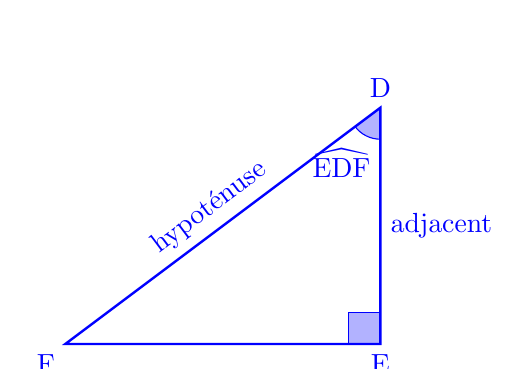
\begin{tikzpicture}[xscale=1,yscale=1,rotate=0,every node/.style={scale=1,rotate=0}]
		\draw[blue, fill=blue!30](4,3)--(4,2.6)node[below left]{$\widehat{\text{EDF}}$}arc(-90:-143.13:0.4)--cycle;
		\draw[blue, fill=blue!30](3.6,0.4)rectangle(4,0);
		\draw[blue, line width=0.3mm](4,0)node[below]{E}--(4,3)node[above]{D}node[midway, right]{adjacent}--(0,0)node[below left]{F}node[midway, above,sloped]{hypoténuse}--cycle;
	\end{tikzpicture}
\end{adjustbox} 
\end{minipage}


Donc  \textbf{réponse B}



\vspace{10mm}
\needspace{10\baselineskip}

% saut de page si moins de 10 lignes disponibles
\section*{\hfill~ DEUXIÈME PARTIE (14 pts)\hfill~}

\section*{Exercice 1 (3 points)}

\begin{enumerate}
	\item Les Pays-Bas ont obtenu 27 médailles d'or.
	\item $63-17-28=18$.
	
L'Australie a obtenu 18 médailles d'or.
	\item La Grande-Bretagne a obtenu 31 médailles de bronze, sur un total de 124.
	
		\begin{tabular}{c|c|c}
		&en nombre  &en \% \\\hline
médailles de bronze		& 31 &$x$  \\\hline
toutes les médailles&124&100\\
	\end{tabular}
	
	
	$x=\dfrac{31\times100}{124}=25$: le pourcentage de médailles de bronze est 25~\%, donc l'affirmation est vraie.
	\item 	\begin{enumerate}
				\item Classons ces nombres par ordre croissant :
				
				56 ~<~ 63 ~<~ 71 ~<~ 75 ~<~ \textcolor{red}{82} ~<~ 89 ~<~ 105 ~<~ 124 ~<~ 220
				
				La médiane est la valeur \og centrale \fg{}, c'est-à-dire la 5\up{ème} : 82 médailles.
				\item Au moins la moitié de ces neuf pays ont eu 82 médailles ou moins de 82 médailles et au moins la moitié ont eu 82 médailles ou plus de 82 médailles.
			\end{enumerate}
	\item 20 médailles représentent nos 100\% de départ.
	
	\(\begin{array}{ccc}
	20 \text{ médailles}& \to & 100\%\\
	26 \text{ médailles}& \to & ?
	\end{array}\)
	
	$?=\dfrac{100\times 26 }{20}=130$.
	
	$130-100=30$
	
	Le nombre de médailles obtenues par le Brésil a augmenté de 30\%.
\end{enumerate}

\needspace{10\baselineskip}
% saut de page si moins de 10 lignes disponibles
\section*{Exercice 2 (4 points)}

\begin{enumerate}
	\item 	\begin{itemize}[label =$\bullet$]
				\item Le côté le plus long est [BC] et $\text{BC}^2=8^2=64$.
				\item D'autre part : $\text{AC}^2+\text{AB}^2=4,8^2+6,4^2=64$.
		\end{itemize}
		Donc $\text{BC}^2=\text{AC}^2+\text{AB}^2$.
		
		D'après la réciproque du théorème de Pythagore, on conclut que le triangle ABC est rectangle en A.
		\item On sait que : 
		\begin{itemize}[label =$\bullet$]
			\item Les points C, A et E d'une part et B, A et D d'autre part, sont alignés dans le même ordre. 
				\item (BC) et (DE) sont parallèles;
		\end{itemize}
		D'après le théorème de Thalès, on a :
		
		\(\begin{array}{ccccc}
		\dfrac{\text{CA}}{\text{AE}}&=&\dfrac{\text{BA}}{\text{AD}}&=&\dfrac{\text{BC}}{\text{DE}}\\
		 & & & & \\
		\dfrac{4,8}{\text{AE}}&=&\dfrac{6,4}{4,8}&=&\dfrac{8}{\text{DE}}\\
		\end{array}\)
		
		Donc $\text{DE}=\dfrac{8\times 4,8}{6,4}=6$ cm,
		
		et $\text{AE}=\dfrac{4,8\times 4,8}{6,4}=3,6$ cm.
		\item Les droites (BC) et (DE) sont parallèles et sont coupées par une sécante (DB), donc les angles alternes-internes formés sont égaux. Ainsi $\widehat{\text{ABC}}=\widehat{\text{ADE}}$.
		\item On sait que $\widehat{\text{ABC}}=\widehat{\text{ADE}}$ et que $\widehat{\text{BAC}}=\widehat{\text{DAE}}$ (ce sont des angles droits).
		
		Donc $\widehat{\text{ACB}}=\widehat{\text{AED}}$.
		
		Ainsi les triangles ABC et ADE ont leurs angles deux à deux de même mesure, les triangles sont donc semblables.
		\item
		L'aire du quadrilatère est la somme des aires des quatre triangles.
		
		 $\mathcal{A}_{\text{BCDE}}=\mathcal{A}_{\text{ABC}}+\mathcal{A}_{\text{ABE}}+\mathcal{A}_{\text{ADE}}+\mathcal{A}_{\text{ADC}}$.
		 
		 Ce sont des triangles rectangles, donc l'aire est la moitié du produit des longueurs des côtés de l'angle droit.
		\begin{itemize}[label =$\bullet$]
			\item $\mathcal{A}_{\text{ABC}}=\dfrac{4,8\times 6,4}{2}=15,36$ cm$^2$.
			\item $\mathcal{A}_{\text{ABE}}=\dfrac{3,6\times 6,4}{2}=11,52$ cm$^2$.
			\item $\mathcal{A}_{\text{ADE}}=\dfrac{4,8\times 3,6}{2}=8,64$ cm$^2$.
			\item $\mathcal{A}_{\text{ADC}}=\dfrac{4,8\times 4,8}{2}=11,52$ cm$^2$.
		\end{itemize}
		Ainsi $\mathcal{A}_{\text{BCDE}}=15,36+11,52+8,64+11,52=47,04$ cm$^2$.
\end{enumerate}
\needspace{10\baselineskip}
% saut de page si moins de 10 lignes disponibles
\section*{Exercice 3 (3 points)}
\subsection*{Partie A}
\begin{enumerate}
	\item On lit sur le graphique que l'image de 3,6 cm par cette fonction est environ 200 cm$^3$.
	\item On lit sur le graphique que l'antécédent de 660 cm$^3$ par cette fonction est environ 5,4 cm.
\end{enumerate}

\needspace{10\baselineskip}
% saut de page si moins de 10 lignes disponibles
\subsection*{Partie B}
\begin{enumerate}
	\item $\mathcal{V}=\dfrac{4}{3}\times \pi\times 2,5^3\approx \np[]{65.45}$: le volume d'une boule, arrondi à l'unité, est d'environ \np[~cm^3]{65}.
	\item $\dfrac{\np{1000}}{65}\approx 15,4$
	
	Donc on peut fabriquer au maximum 15 boules avec \np[~cm^3]{1000} de plastique.
	\item 
	\begin{tabular}{c|c|c}
	masse en g& \np{0.9} &$x$ \\\hline
	volume en cm\up{3}& 1 &65  \\
\end{tabular}

	$0,9\times 65= 58,5$ g.
	
	Donc la masse d'une boule est d'environ \np[~g]{59}. %arrondir à l'entier car 65 est déjà arrondi à l'entier
\end{enumerate}

\needspace{10\baselineskip}
% saut de page si moins de 10 lignes disponibles
\section*{Exercice 4 (2 points)}
\begin{enumerate}
	\item $112\div 16=7$ et $140\div 16 =8,75$
	
	140 n'est pas divisible par 16, donc on ne peut pas constituer 16 sachets.
	\item \begin{align*}
	140&=2\times 70\\
	&=2\times 2\times 35\\
	&=2\times 2\times 5\times 7
	\end{align*}
	Donc la décomposition en produit de facteurs premiers de 140 est $2^2\times 5\times 7$.
	\item Grâce à leurs décompositions en produit de facteurs premiers, on remarque que 112 et 140 sont tous les deux divisibles par $2^2\times 7$ c'est-à-dire 28 ; et que c'est le plus grand diviseur commun de ces deux nombres.
	
	Le nombre maximum de sachets ayant la même composition qu'on peut constituer en utilisant tous les bonbons est donc de 28 sachets.
	
	$112\div 28 =4$ et $140\div 28=5$.
	
	Dans chaque sachet, il y aura 4 bonbons à la fraise et 5 bonbons au caramel.
\end{enumerate}
\needspace{10\baselineskip}
% saut de page si moins de 10 lignes disponibles
% Fin du document
\end{document}